%%%%%%%%%%%%%%%%%%%%%%%%%%%%%%%%%%%%%%%%%%%%%%%%%%%%%%%%%%%%
\documentclass[11pt,            % Schriftgröße {{{
               a4paper,         % A4
               oneside,         % Einseitig
               DIV12,           % Papiergröße
             % DIV15,           % Größer
             % draft,           % Entwurf
               fleqn,           % Linksbündige Gleichungen
             % headsepline,     % Trennlinie oben
             % footsepline,     % -""-       unten
             % smallheadings,   % Kleine Überschriften
             % pointlessnumbers,% Keine Punkte
               halfparskip,     % Halbe Zeile Absatz statt Einzug
               nochapterprefix, % Kein "Kapitel"
             % bibtotoc         % "Literatur" im TOC  oder
               bibtotocnumbered,% -""-, nummeriert
             % idxtotoc,        % Index im TOC
              ]{scrartcl} %%% }}}
%%%%%%%%%%%%%%%%%%%%%%%%%%%%%%%%%%%%%%%%%%%%%%%%%%%%%%%%%%%%

%%%%%%%%%%%%%%%%%%%%%%%%%%%%%%%%%%%%%%%%%%%%%%%%%%%%%%%%%%%%
%%% Pakete {{{
\usepackage[utf8]{inputenc}         % Umlaute etc.
\usepackage[T1]{fontenc}            % T1-kodierte Fonts
%\usepackage{ae,aecompl}             % Kodierung für PDF
%\usepackage{ngerman}                % Deutsche Trennungen,
                                    % dt. Begriffe
\usepackage{setspace}               % Single- oder Onehalfspacing
\setcounter{tocdepth}{4}            % 4 Hirarchien im Inhaltsv.
\usepackage{times}                  % Times als Schrift
\usepackage{amsmath,amssymb,amstext}% Mathematische Symbole
\usepackage{exscale}                % Skalierung von Summen-c und Int.-zeichen
\usepackage{url}                    % Darstellung von URLs
\usepackage{calc}

%%% Optional, je nach Dokument
% \usepackage{listings}             % Quelltext-Listings
% \usepackage{units}                % Technische Units
% \usepackage{psfrag}               % Ersetzts PS-Schriften
  \usepackage{color}                % Farben in LaTeX
% \usepackage{floatflt}             % Textumflossene Bilder...
% \usepackage{picins}               % Textumflossene Bilder
  \usepackage{textcomp}             % Spezielle Zeichen
  \usepackage{gensymb}              % Spezielle Zeichen
% \usepackage{eurosym}              % Euro-Symbol
% \usepackage{currvita}             % Befehle für CVs
  \usepackage{ifpdf}                % Wird ein PDF erstellt?

% https://tex.stackexchange.com/questions/37581/latex-figures-side-by-side
  \usepackage{caption}
  \usepackage{subcaption}

%%% Layout
\usepackage{scrpage2}               % KOMA-Überschriften und -Fußzeilen.
%%% }}}
%%%%%%%%%%%%%%%%%%%%%%%%%%%%%%%%%%%%%%%%%%%%%%%%%%%%%%%%%%%%

%%%%%%%%%%%%%%%%%%%%%%%%%%%%%%%%%%%%%%%%%%%%%%%%%%%%%%%%%%%%
%%% PDF {{{

\ifpdf
  \usepackage[pdftex]{graphicx}
  \usepackage{float}
  \DeclareGraphicsExtensions{.pdf}
  \pdfcompresslevel=9
  \usepackage[%
    pdftex=true,
    backref=true,
    colorlinks=true,
    bookmarks=true,
    breaklinks=true,
    linktocpage=true,
    bookmarksopen=false,
    bookmarksnumbered=false,
    pdfpagemode=None
  ]{hyperref}
  \hypersetup{
    pdftitle={},
    pdfauthor={Julius Plenz},
    pdfsubject={},
    pdfcreator={LaTeX2e and pdfLaTeX},
    pdfproducer={},
    pdfkeywords={}
  }
\else
  \usepackage[dvips]{graphicx}
  \DeclareGraphicsExtensions{.eps}
  % \usepackage[%
  %   dvips,
  %   breaklinks=true,
  %   colorlinks=false
  % ]{hyperref}
\fi

%%% }}}
%%%%%%%%%%%%%%%%%%%%%%%%%%%%%%%%%%%%%%%%%%%%%%%%%%%%%%%%%%%%

%%%%%%%%%%%%%%%%%%%%%%%%%%%%%%%%%%%%%%%%%%%%%%%%%%%%%%%%%%%%
%%% Eigene Funktionen {{{
%%% Beispiel:  \bild{200pt}{foo}{That's a foo\ldots}
\newcommand{\bild}[3]{
  \begin{figure}
    \includegraphics[width=#1, keepaspectratio=true]{#2}
    \caption{#3}
    \label{#2}
  \end{figure}
}

%% \floatimg{filename}{caption+label}{r/l}{8cm}
\newcommand{\floatimg}[4]{
  \piccaption{#2}
  \parpic[#3]{\includegraphics[width=#4]{#1}}
}
%%% }}}
%%%%%%%%%%%%%%%%%%%%%%%%%%%%%%%%%%%%%%%%%%%%%%%%%%%%%%%%%%%%

%%%%%%%%%%%%%%%%%%%%%%%%%%%%%%%%%%%%%%%%%%%%%%%%%%%%%%%%%%%%
%%% Pagestyle {{{
  \pagestyle{scrheadings}
% \pagestyle{fancyhdrs}
% \pagestyle{empty}
%%% }}}
%%%%%%%%%%%%%%%%%%%%%%%%%%%%%%%%%%%%%%%%%%%%%%%%%%%%%%%%%%%%

%%%%%%%%%%%%%%%%%%%%%%%%%%%%%%%%%%%%%%%%%%%%%%%%%%%%%%%%%%%%
%%% Seitenkopf- und -Fußzeilen {{{
 \automark[subsection]{section} % \left- und \rightmark bekommen Inhalt
%%% Oben: Links, Mitte, Rechts
 \ihead[]{\rightmark}
 \chead[]{}
 \ohead[]{\pagemark}
%%% Unten: Links, Mitte, Rechts
 \ifoot[]{}
 \cfoot[]{}
 \ofoot[]{}
%%% }}}
%%%%%%%%%%%%%%%%%%%%%%%%%%%%%%%%%%%%%%%%%%%%%%%%%%%%%%%%%%%%

%%%%%%%%%%%%%%%%%%%%%%%%%%%%%%%%%%%%%%%%%%%%%%%%%%%%%%%%%%%%
%%% Sonstiges {{{
% \setlength{\parindent}{17pt}      % Einzug 17pt,
% \setlength{\parskip}{2pt}         % keine Leerzeilen.

% \textwidth      127mm             % Textbreite
% \textheight     235mm             % Texthöhe
% \topmargin     -5mm               % Abstand oben
% \oddsidemargin  7mm               % Abstand Links, onepage

%\onehalfspacing                    % Zeilenabstand: Bei korrektur,
 \singlespacing                     % bei Abgabe

% Punkt- und Komma Abstände bei Tausendern/
% Dezimalzahlen ans deutsche anpassen!
 \mathcode`,="013B
 \mathcode`.="613A

 \setlength{\emergencystretch}{2em} % Notfallsstreckung
 \addtolength{\voffset}{10pt}

% Kommandoänderungen
%\renewcommand{\figurename}{Abb.} % Bildunterschriften: Abb. anstatt Fig.
%\renewcommand*{\cvheadingfont}{\raggedleft\Huge\bfseries} % CV: Überschriften
%%% }}}
%%%%%%%%%%%%%%%%%%%%%%%%%%%%%%%%%%%%%%%%%%%%%%%%%%%%%%%%%%%%


\usepackage{amsthm}

\theoremstyle{definition}
\newtheorem*{beweis}{Beweis}
\newtheorem{definition}{Definition}
\newtheorem*{bemerkung}{Bemerkung}
\newtheorem*{beispiel}{Beispiel}


\begin{document}

%%%%%%%%%%%%%%%%%%%%%%%%%%%%%%%%%%%%%%%%%%%%%%%%%%%%%%%%%%%%
%%% Titelseite {{{
%\pagenumbering{none}                % Für die Titelseite: Keine Seitennummern,
%\thispagestyle{empty}               % keine Kopf- und Fußzeilen.
%
%\begin{center}
%
%\end{center}
%\newpage
%
%%% }}}
%%%%%%%%%%%%%%%%%%%%%%%%%%%%%%%%%%%%%%%%%%%%%%%%%%%%%%%%%%%%

%%%%%%%%%%%%%%%%%%%%%%%%%%%%%%%%%%%%%%%%%%%%%%%%%%%%%%%%%%%%
%%% Inhaltsverzeichnis {{{
  \pagenumbering{arabic}            % Arabische Nummerierung
% \pagenumbering{roman}             % Kleine, römische Nummerierung
% \tableofcontents                  % Das Inhaltsverzeichnis
% \listoffigures                    % Verzeichnis aller Abbildungen
% \listoftables                     % Verzeichnis aller Tabellen
% \pagenumbering{arabic}            % ...und wieder Arabisch
% \newpage
%%% }}}
%%%%%%%%%%%%%%%%%%%%%%%%%%%%%%%%%%%%%%%%%%%%%%%%%%%%%%%%%%%%

%%%%%%%%%%%%%%%%%%%%%%%%%%%%%%%%%%%%%%%%%%%%%%%%%%%%%%%%%%%%
%%% Inhalt {{{


\section*{Introduction}

In this project we will introduce the \emph{Petersen graph} and highlight
some of its interesting properties, explain the construction of the
\emph{cross cap} and proceed to show how to embed the Petersen graph
onto the suface of the cross cap without any edge intersection --
an embedding that is not possible to achieve in the plane.

Using these results, we will subsequently create a video
using the software \emph{Maya} that visualizes the important aspects
of this construction. In particular, this visualizations can be
understood also by non-mathematicians.

\section{Theoretical preliminaries}

We will first explore the construction of the Petersen graph and the
cross cap, highlighting interesting properties. We will then proceed
to motivate the embedding of the Petersen graph on the surface of the
cross cap.

\subsection{The Petersen Graph}

The Petersen Graph is an important example from graph theory that has
proven to be useful in particular as a counterexample.

\begin{definition}[Kneser graph]
  The \emph{Kneser graph of n, k} (denoted $KG_{n,k}$) consists of
  the $k$-element subsets of $\{1,\ldots,n\}$ as vertices, where an
  edge connects two vertices if and only if the two sets corresponding
  to the vertices are disjoint.
\end{definition}

This graph is ${n-k}\choose k$-regular and has a chromatic number of
$n - 2k + 2$ \cite{kneser}. A special case is the Petersen graph $P =
KG_{5,2}$, called so after the Danish mathematician Julius Petersen
(1839--1910). See figures \ref{fig:petersen} and
\ref{fig:petersen-twointersect}.

\begin{figure}[p]
  \begin{subfigure}[t]{.45\textwidth}
    \centering
    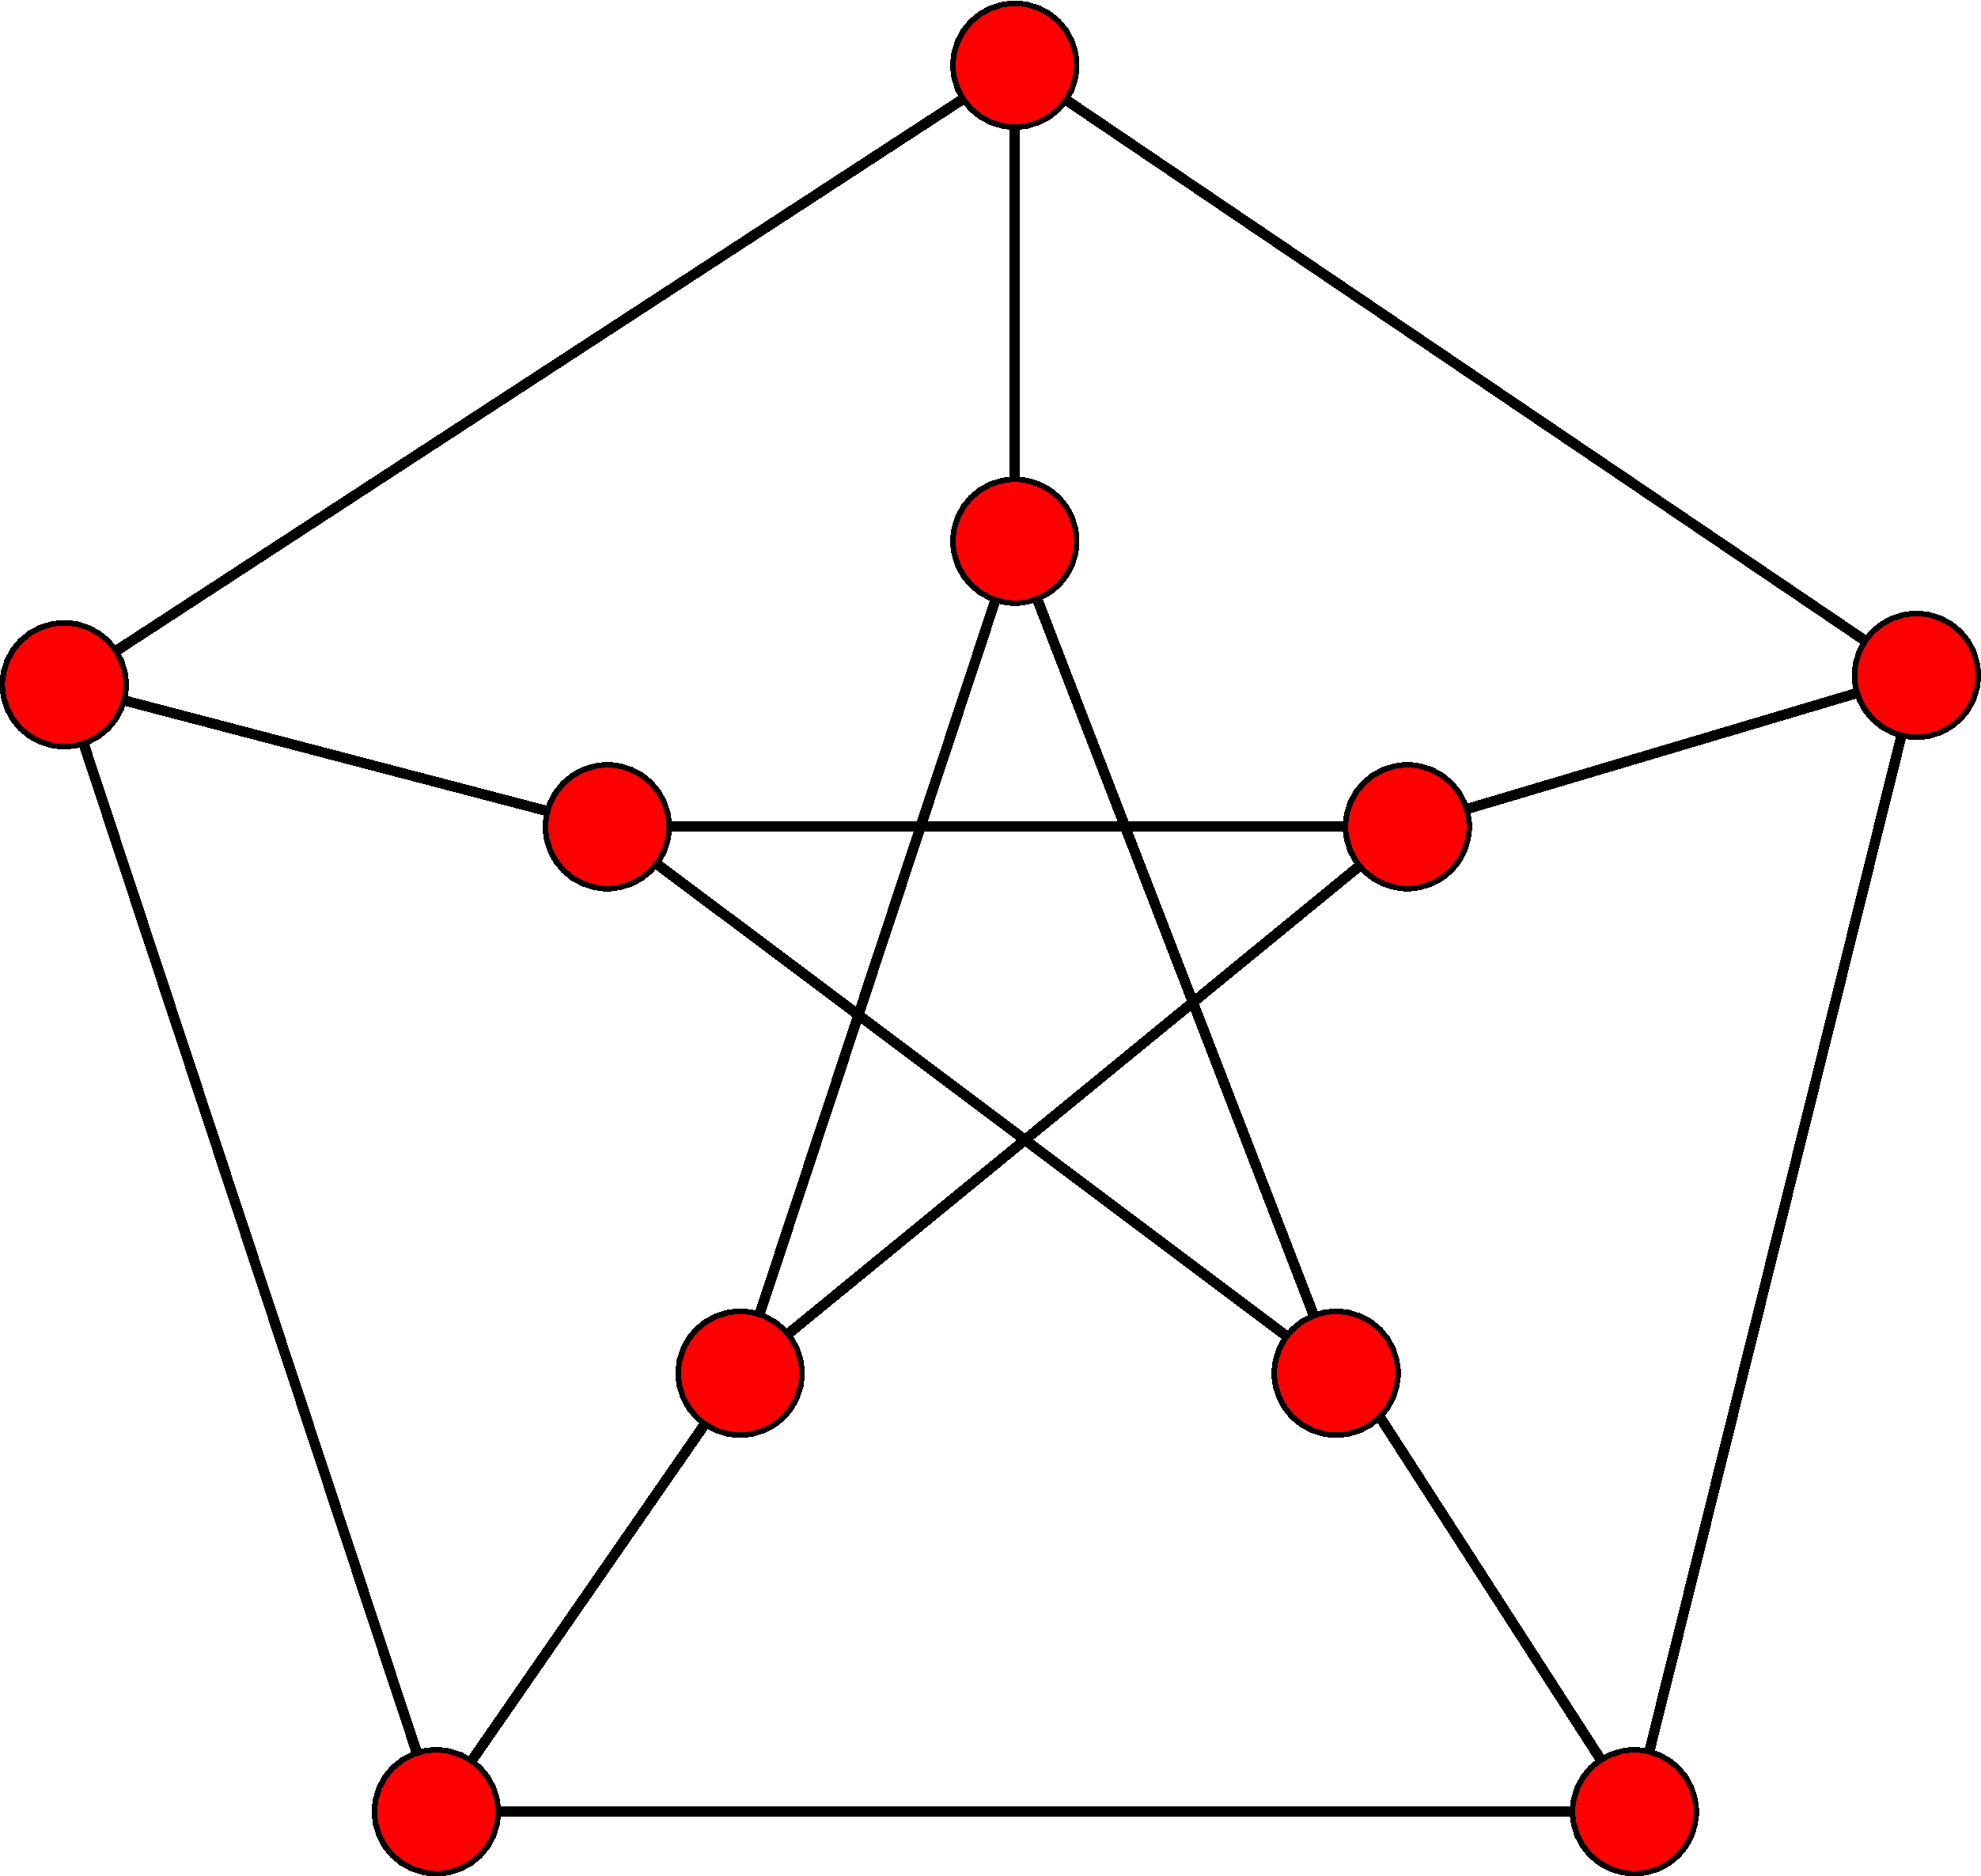
\includegraphics[keepaspectratio=true,width=\textwidth]{../planar-graphs/petersen-grundlage.pdf}
    \caption{Traditional realization of the Petersen graph in the plane.
      The inner vertices and their edges form a pentagram; the outer
      vertices form a pentagon. This version exhibits five edge
      intersections.}
    \label{fig:petersen}
  \end{subfigure}\hfill
  \begin{subfigure}[t]{.45\textwidth}
    \centering
    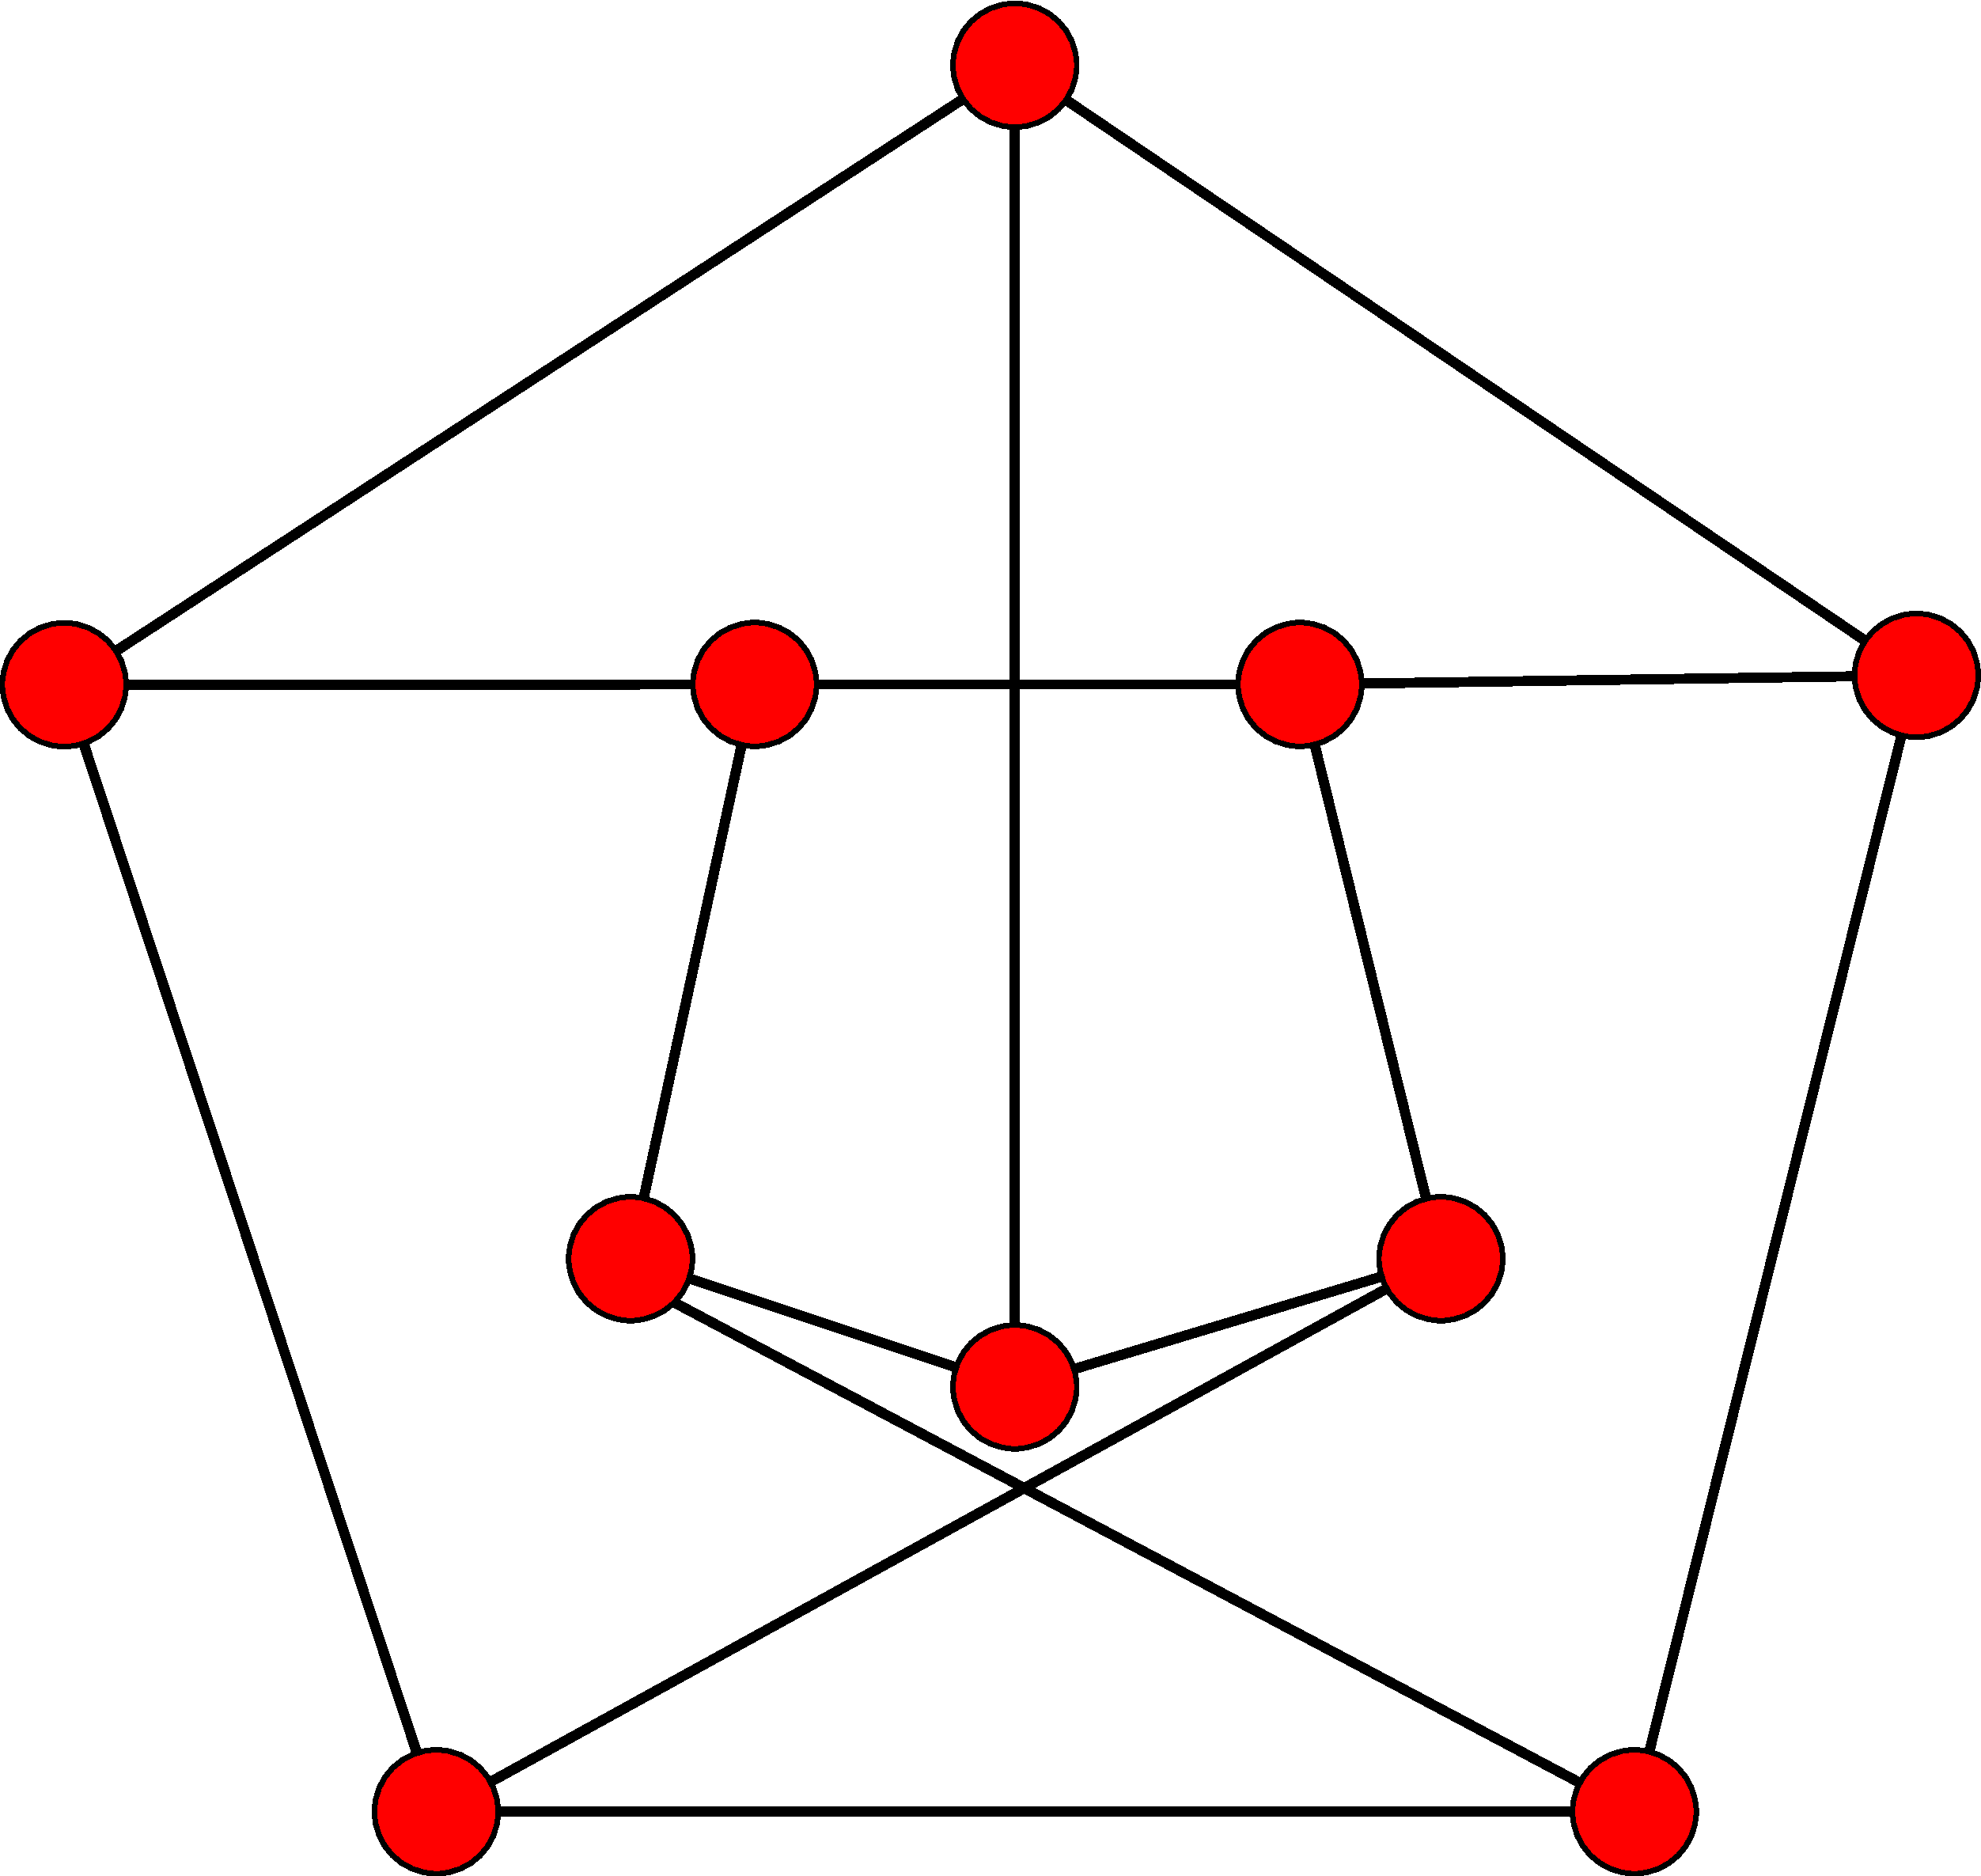
\includegraphics[keepaspectratio=true,width=\textwidth]{../planar-graphs/petersen-zweikreuzungen.pdf}
    \caption{The Petersen graph in the plane with just two edge
      intersections. It can be shown that this is the minimum number of
      intersections necessary when drawing the graph in the plane.}
    \label{fig:petersen-twointersect}
  \end{subfigure}
  \caption{Two drawings of the Petersen graph in the plane}
\end{figure}

The Petersen graph has the following interesting properties \cite{petersen}:

\begin{itemize}
  \item It has chromatic number $n - 2k + 2 = 3$, so an optimal vertex
    coloring needs at least three different colors (see figure
    \ref{fig:color-vertex})
  \item It has chromatic index 4, meaning a minimum edge coloring must
    use at least four different colors (see \ref{fig:color-edge})
  \item It is the smallest (and until 1946 the only known)
    \emph{snark} -- that is, a connected, bridgeless cubic graph with
    chromatic index 4
\end{itemize}

\begin{figure}[p]
  \begin{subfigure}[t]{.45\textwidth}
    \centering
    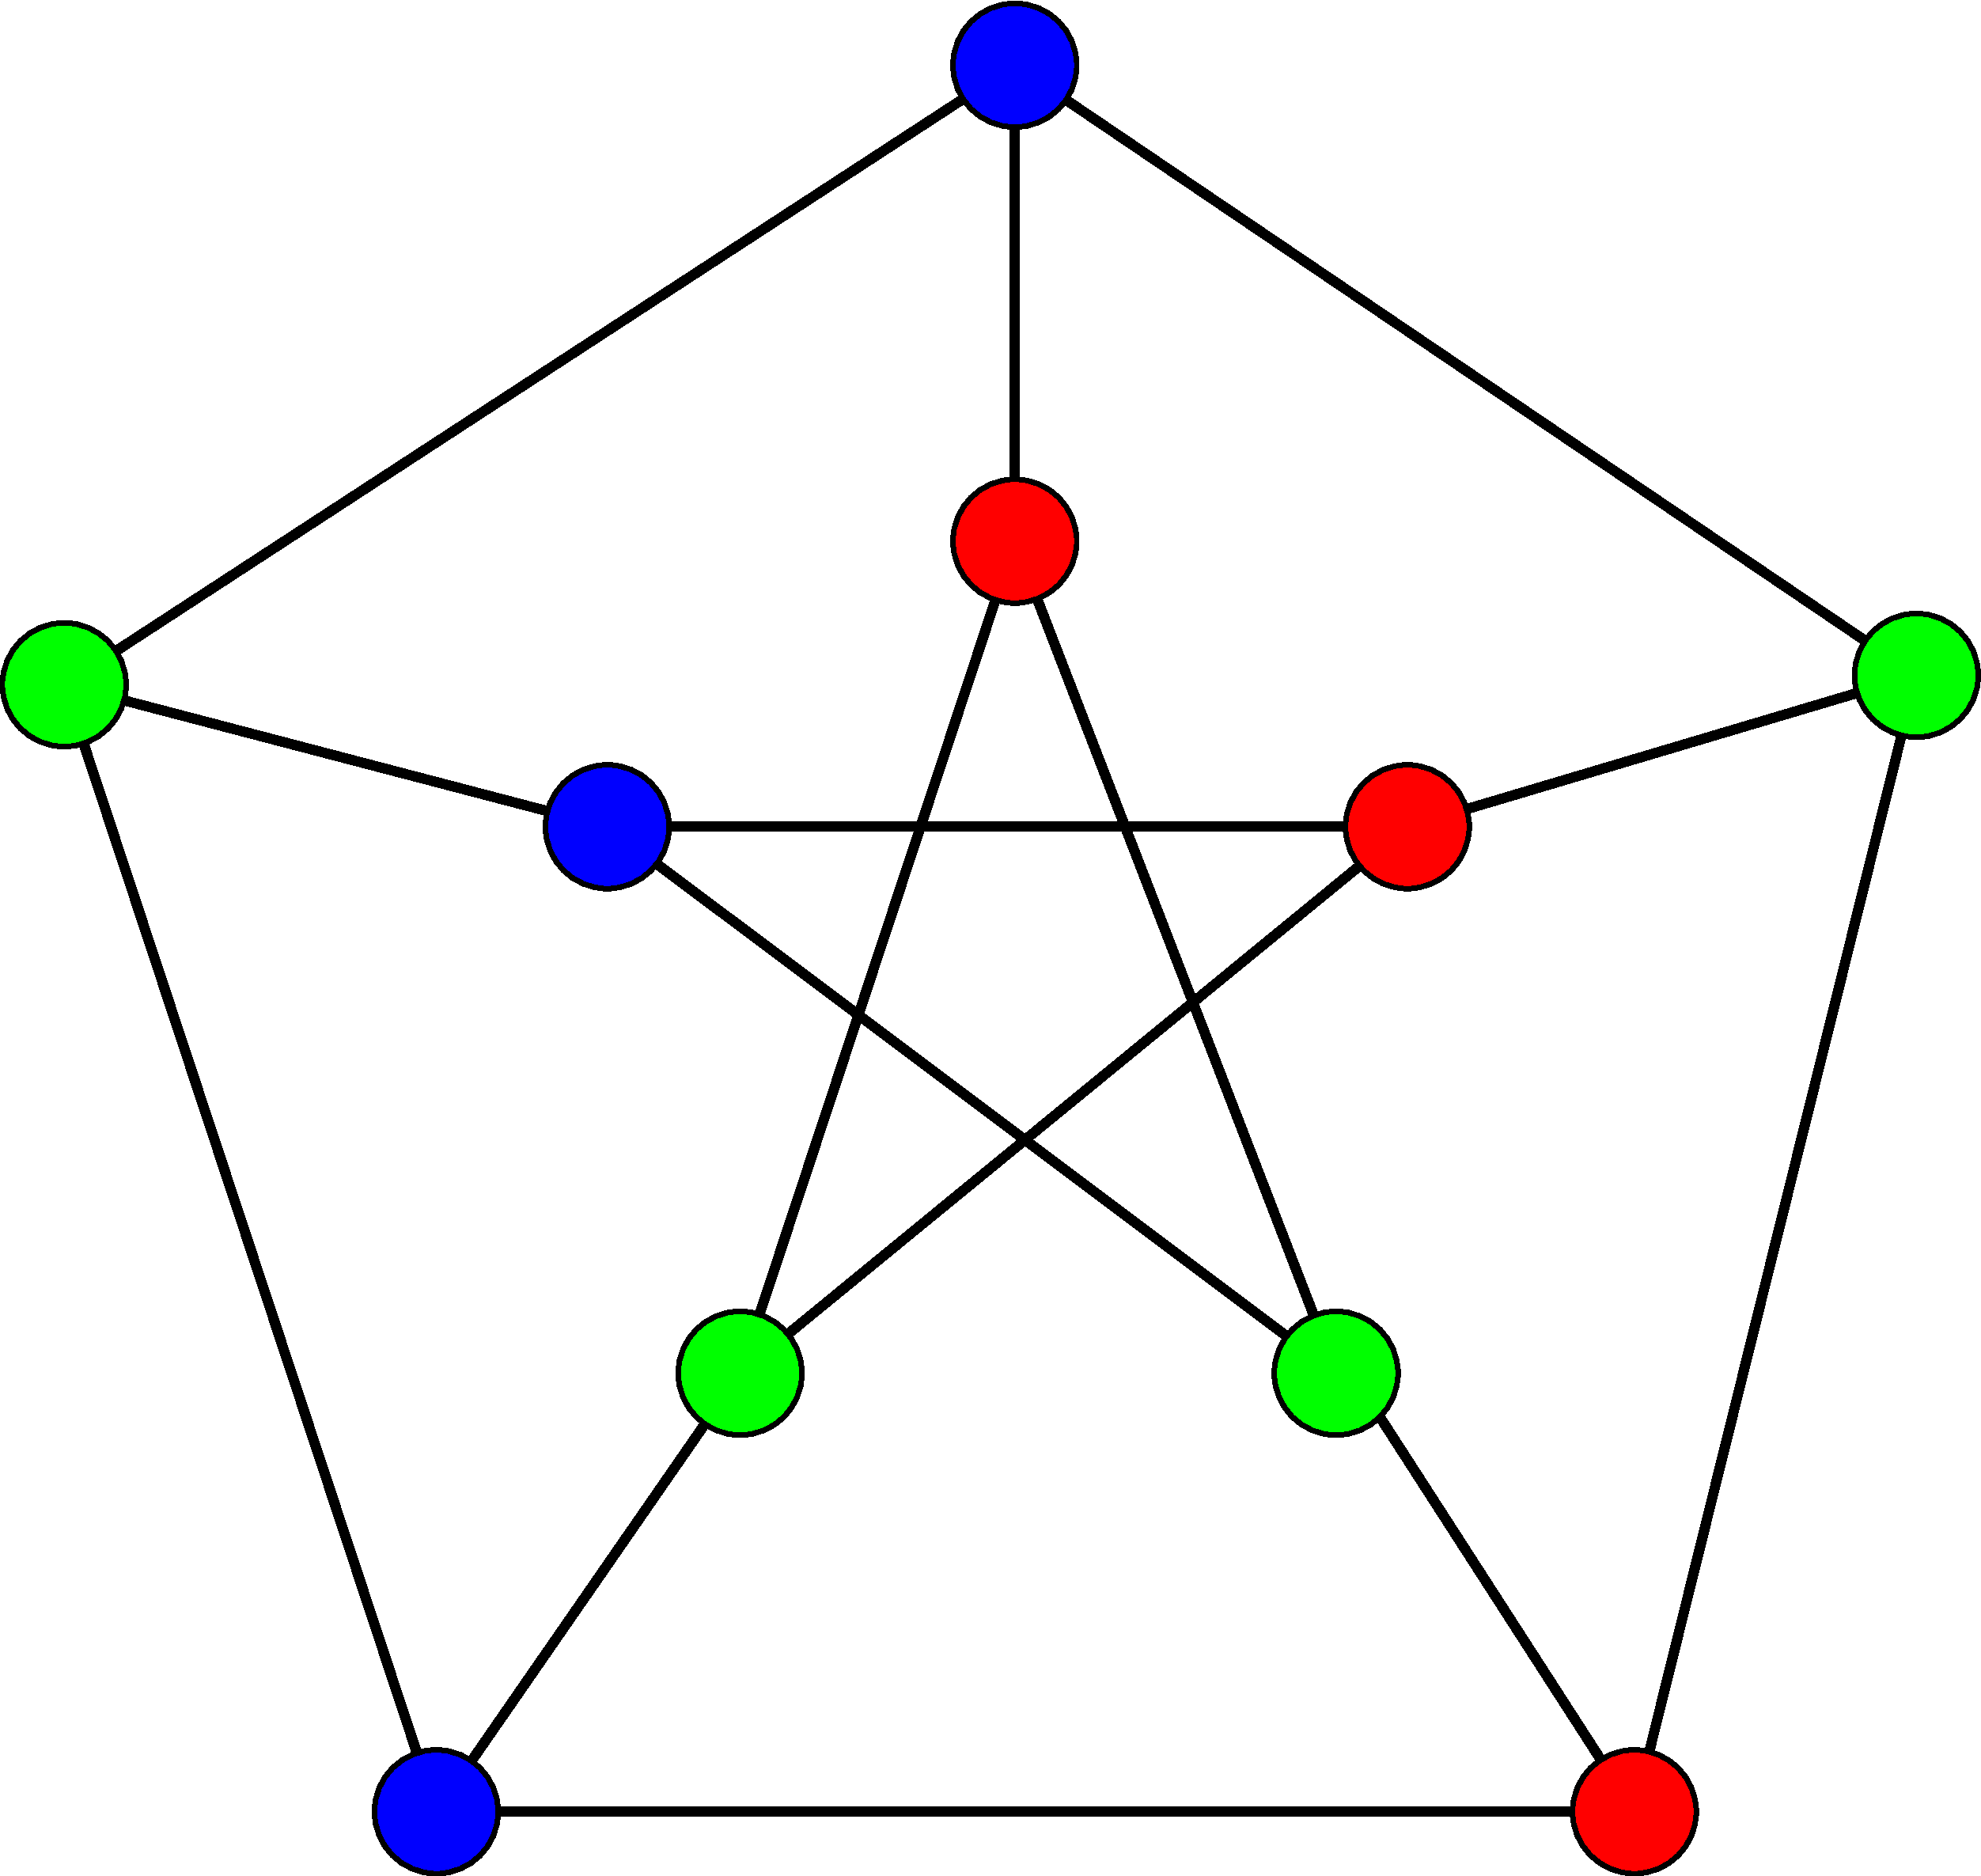
\includegraphics[keepaspectratio=true,width=\textwidth]{../planar-graphs/petersen-vertex-threecoloring.pdf}
    \caption{A vertex 3-coloring of the Petersen graph}
    \label{fig:color-vertex}
  \end{subfigure}\hfill
  \begin{subfigure}[t]{.45\textwidth}
    \centering
    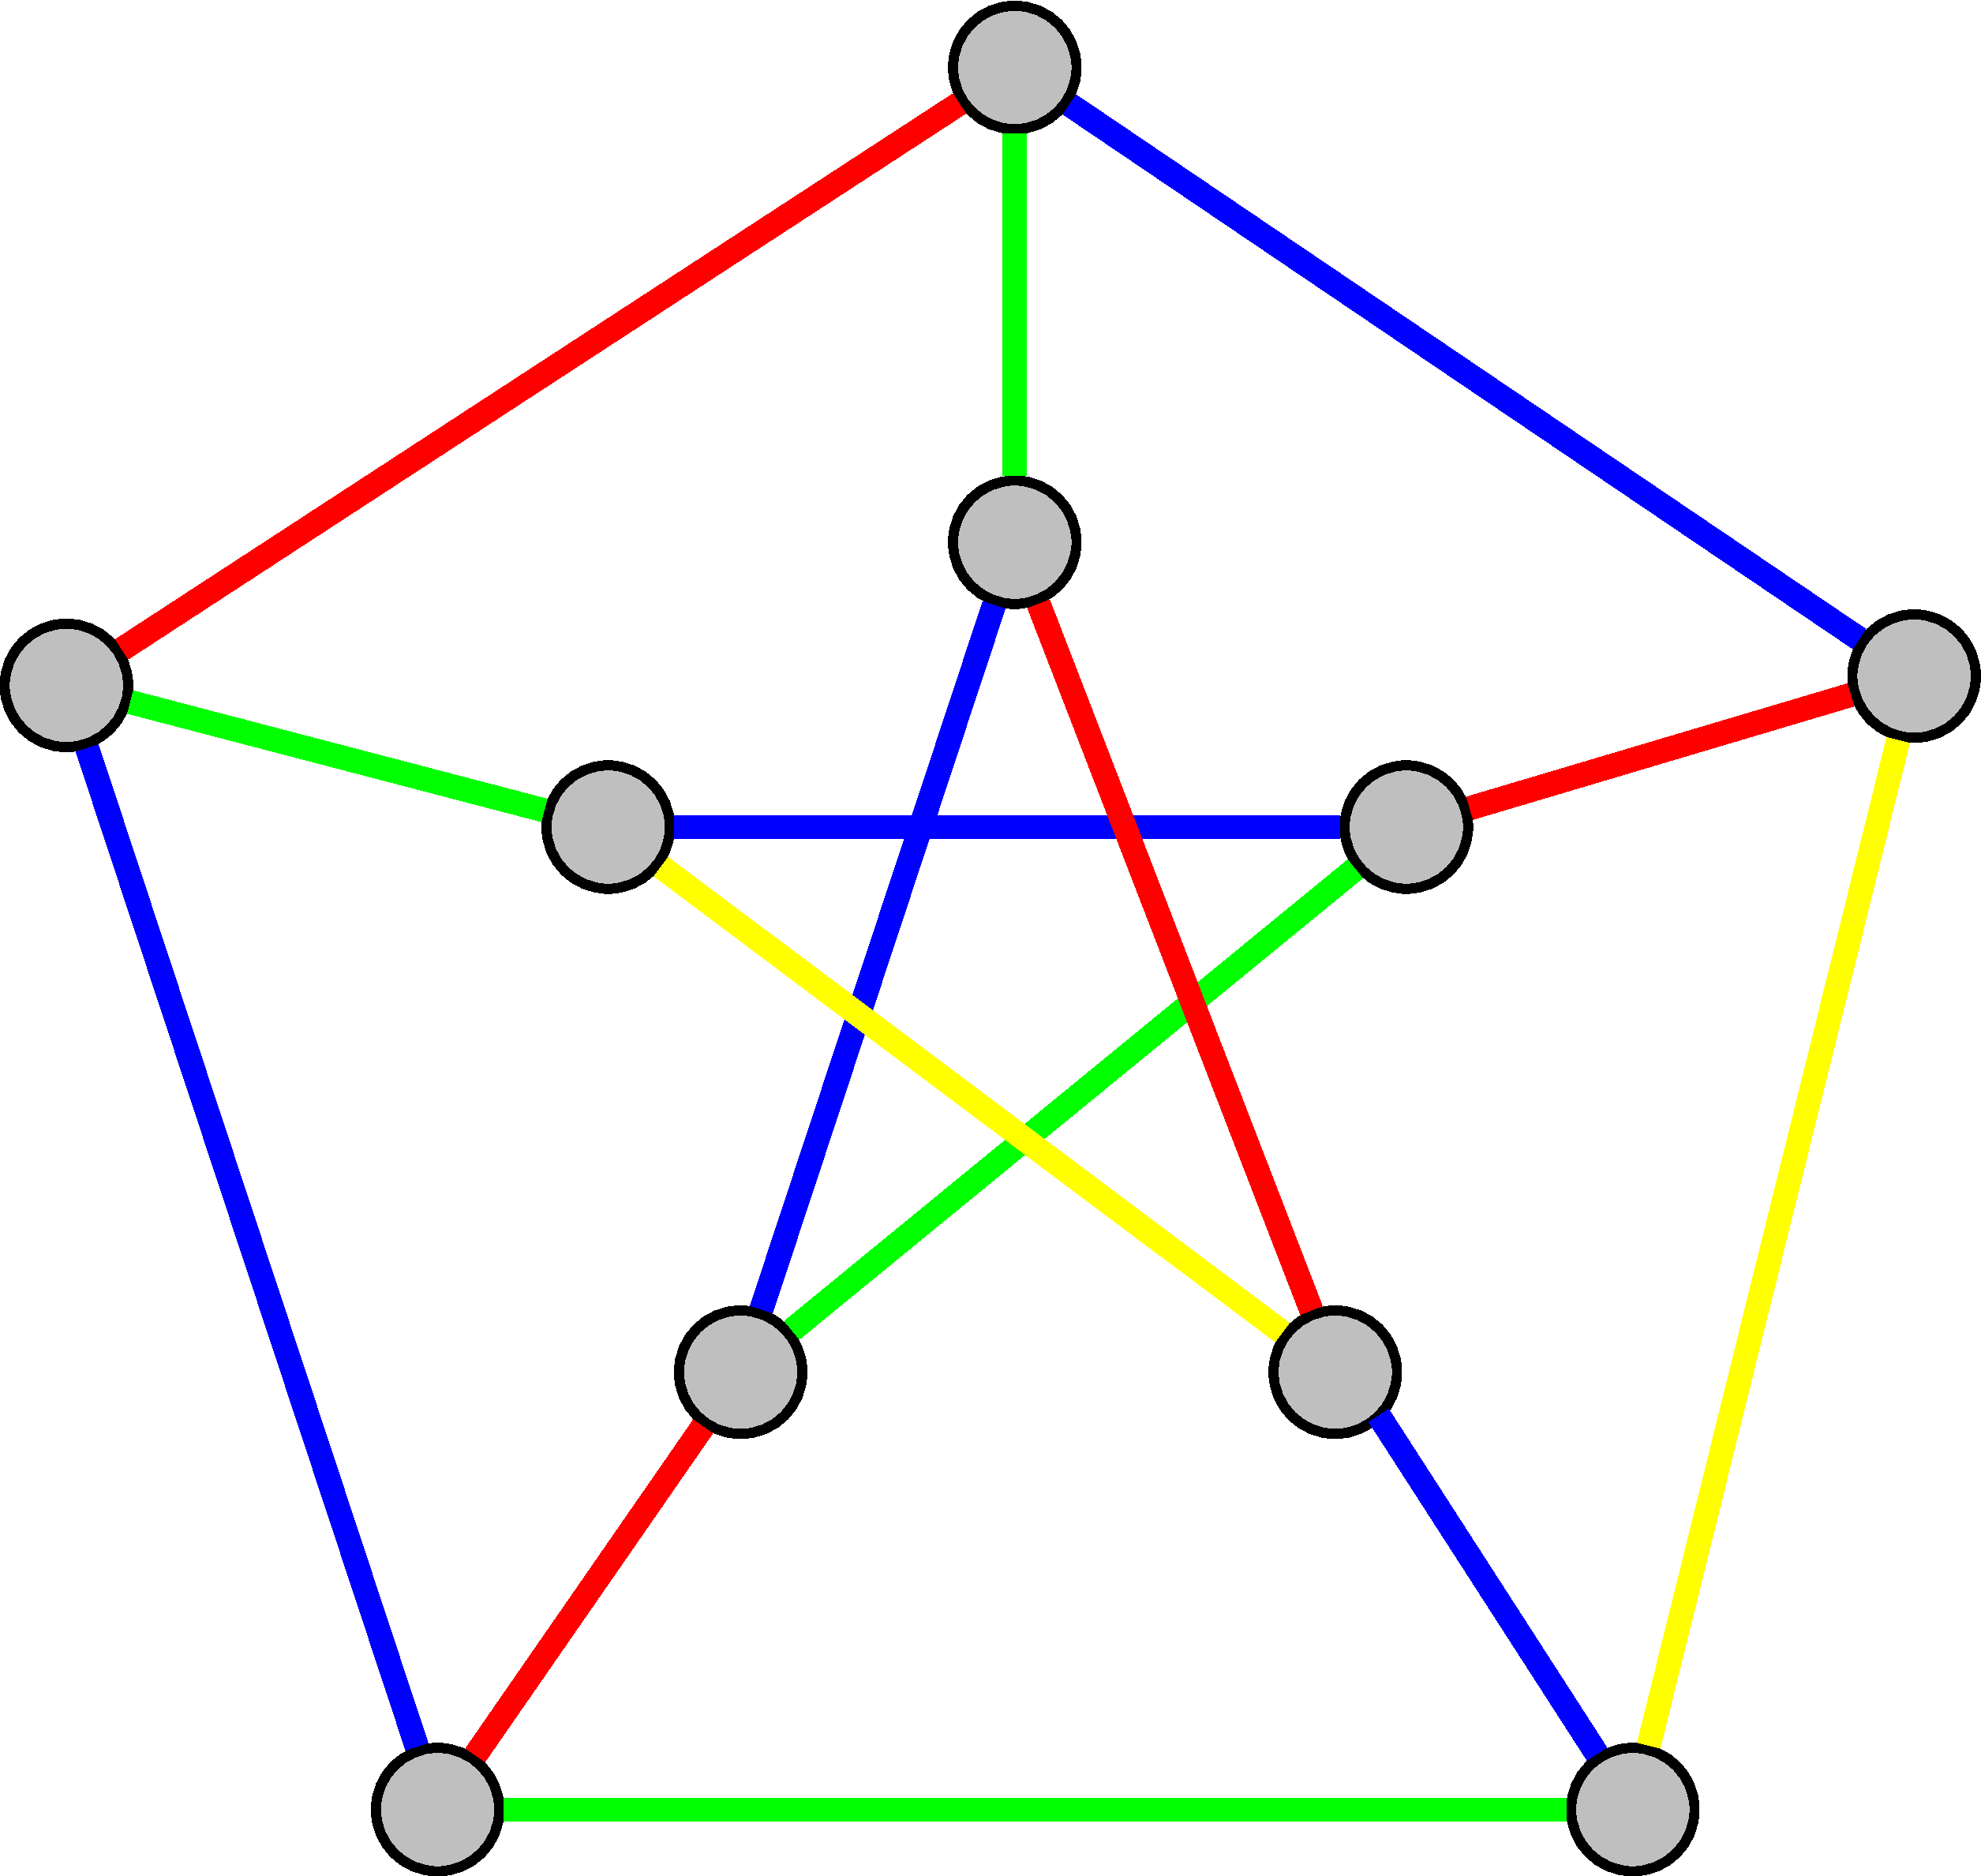
\includegraphics[keepaspectratio=true,width=\textwidth]{../planar-graphs/petersen-edge-fourcoloring.pdf}
    \caption{An edge 4-coloring of the Petersen graph}
    \label{fig:color-edge}
  \end{subfigure}
  \caption{The Petersen graph has chromatic number 3 and chromatic index 4}
\end{figure}

The Petersen graph has crossing number $\operatorname{cr}(P) = 2$,
meaning it cannot be embedded into the plane with less than 2 edge
intersections \cite[p.~2]{crossingnr}. It can, however, be embedded
without any edge intersections on the surface of the cross cap.

\subsection{The Cross Cap}

\begin{minipage}{0.55\textwidth}
  The cross cap is a two-dimensional real manifold that is homeomorphic
  tho the real projective plane $\mathbb{R}P^2$.

  \begin{definition}[Real projective space]
    The \emph{real projective space} $\mathbb{R}P^n$ consists of the lines
    passing through the origin of $\mathbb{R}^{n+1}$. In the case $n=1$,
    this is called the \emph{real projective line}; in the case $n=2$,
    \emph{real projective plane}.
  \end{definition}

  An equivalent (and more intuitive) construction for $\mathbb{R}P^n$
  can be given by identifying antipodal points of $S^n$. Hence, the real
  projective plane is topologically equivalent to $D^2$ with antipodal
  points at the border identified (see figure \ref{fig:rp2}).
\end{minipage}%
\hfill%
\begin{minipage}{0.35\textwidth}
  \begin{figure}[H]
    \centering
    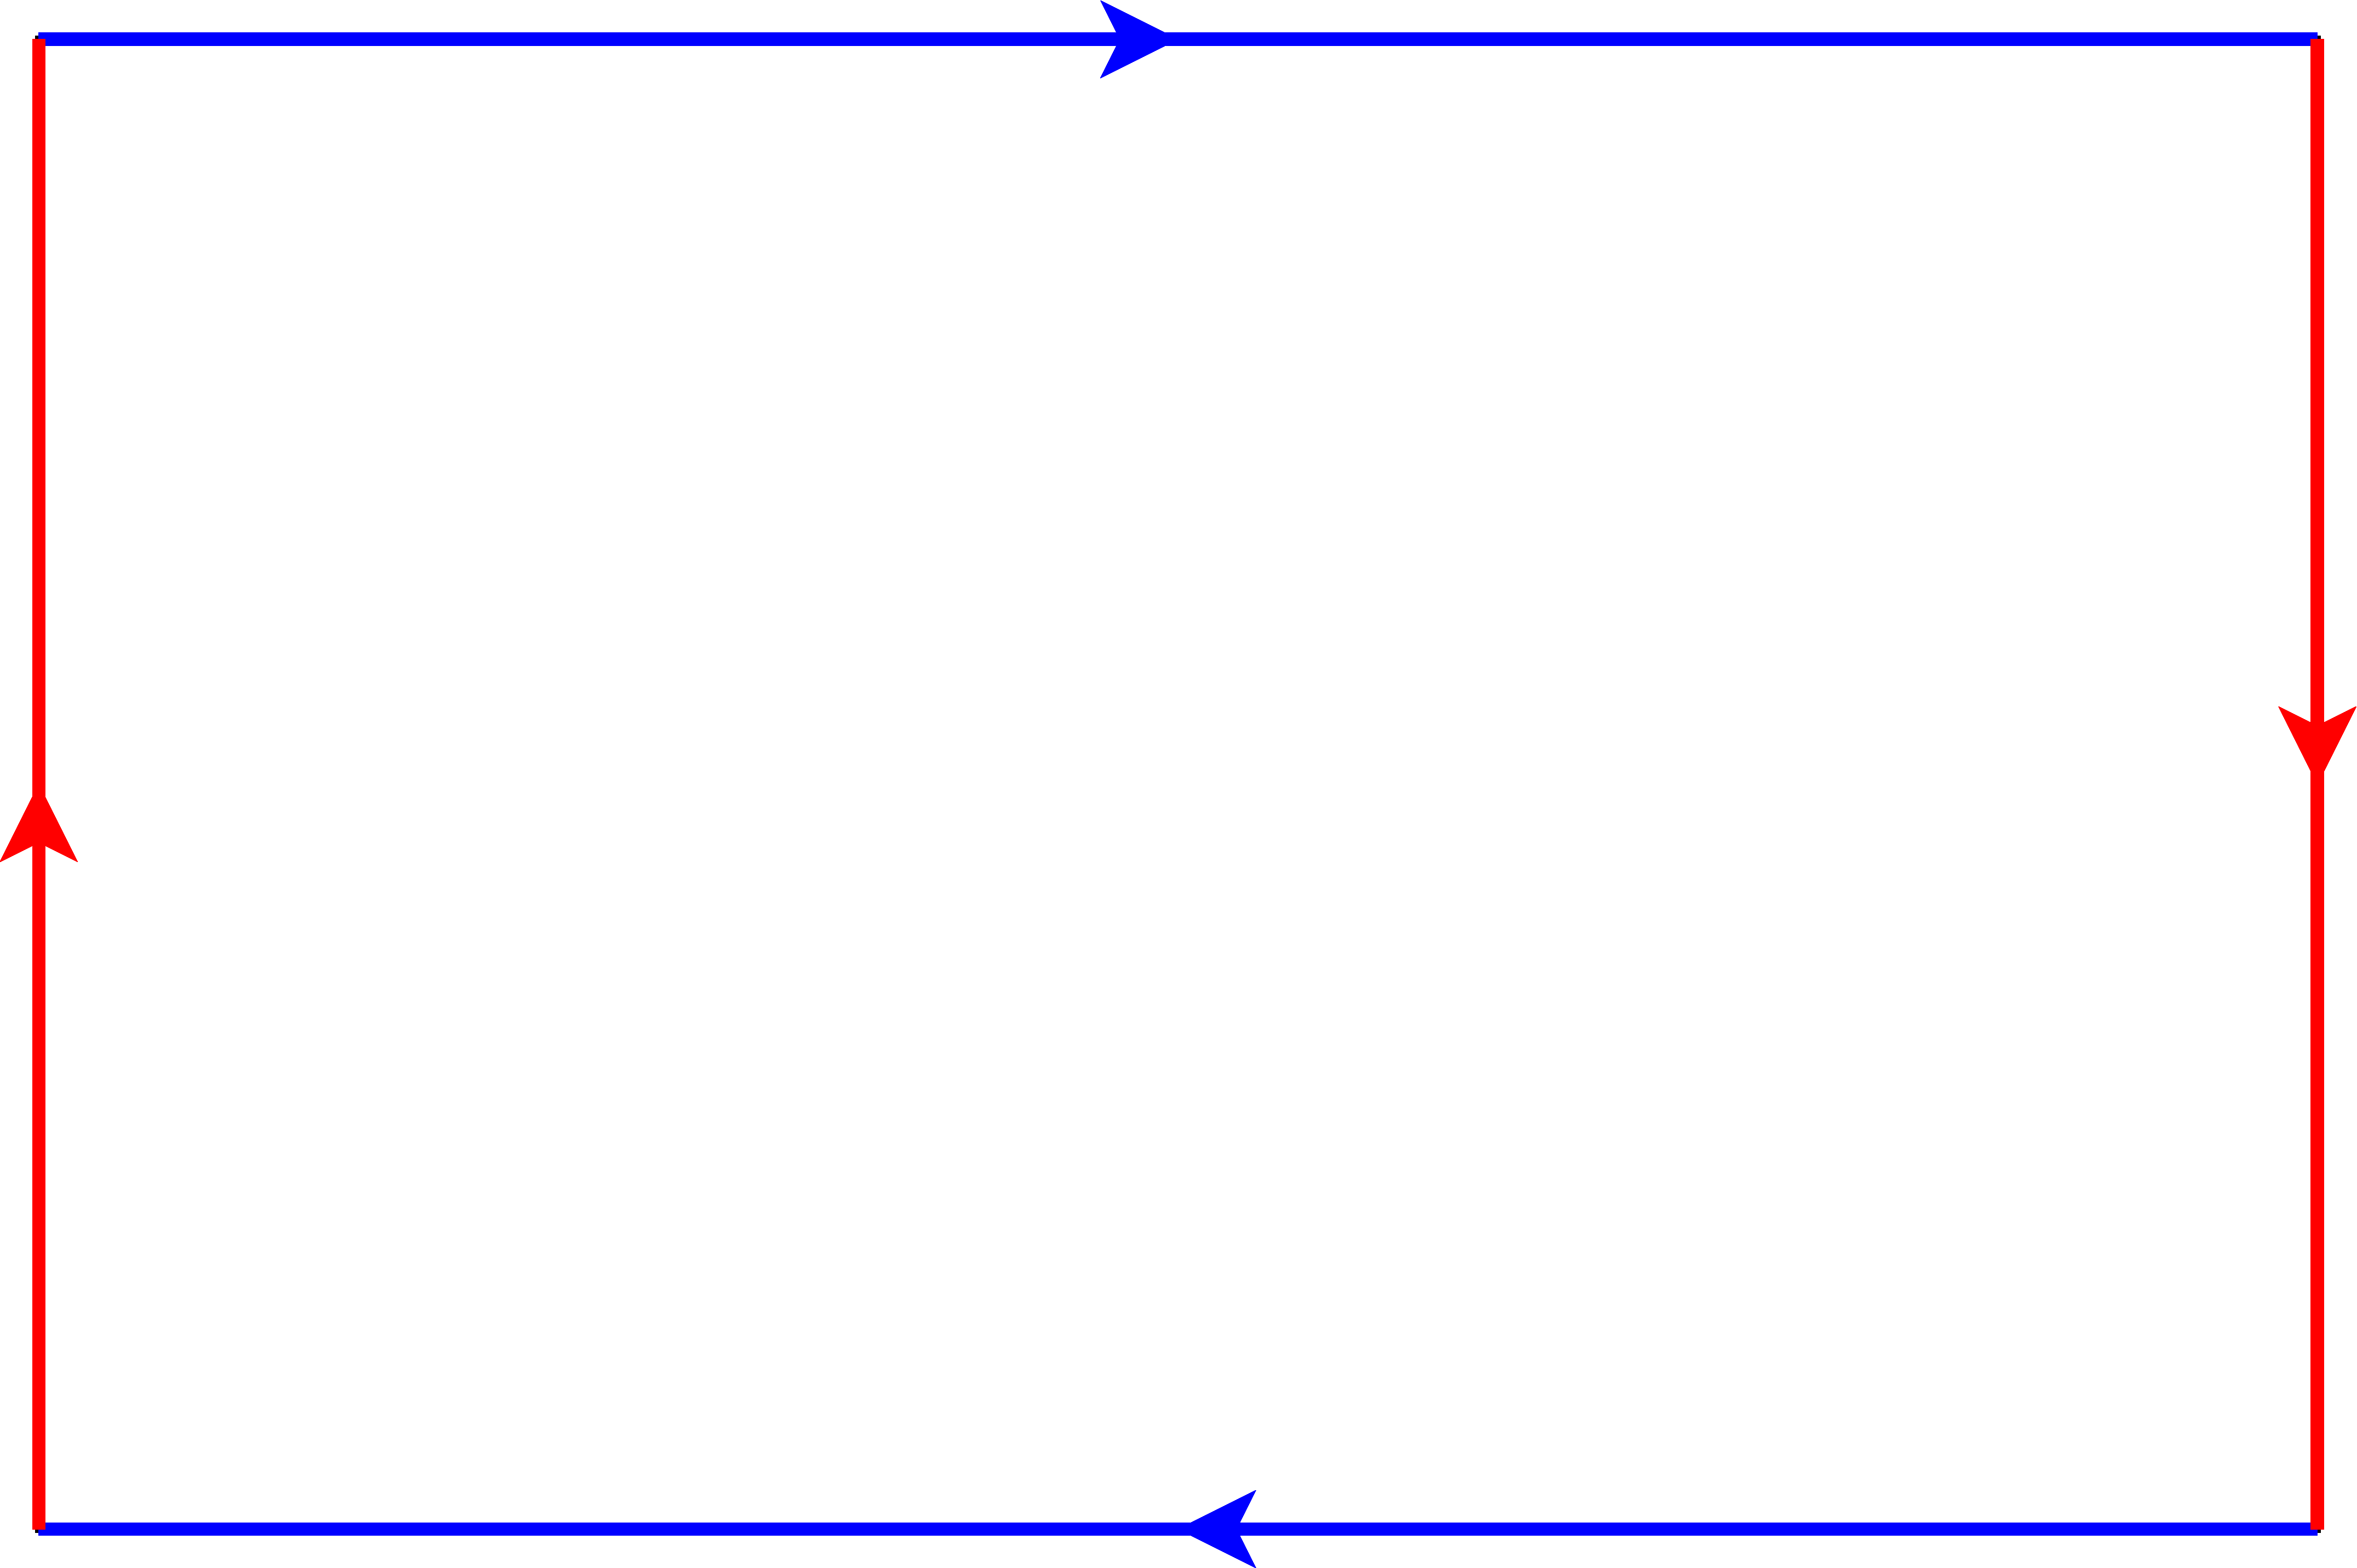
\includegraphics[keepaspectratio=true,width=\textwidth]{../planar-graphs/crosscap-construction.pdf}
    \caption{The topological view: How to glue $[0,1]\times[0,1]$
      together to construct the real projective plane.}
    \label{fig:rp2}
  \end{figure}
\end{minipage}%

\subsection{Embedding the Petersen graph on the cross cap}

Using this “planar model” of $\mathbb{R}P^2$, we can now easily see
that an embedding of the Petersen graph without edge intersection
onto the surface of the cross cap is in fact possible:

\begin{figure}[h]
  \centering
  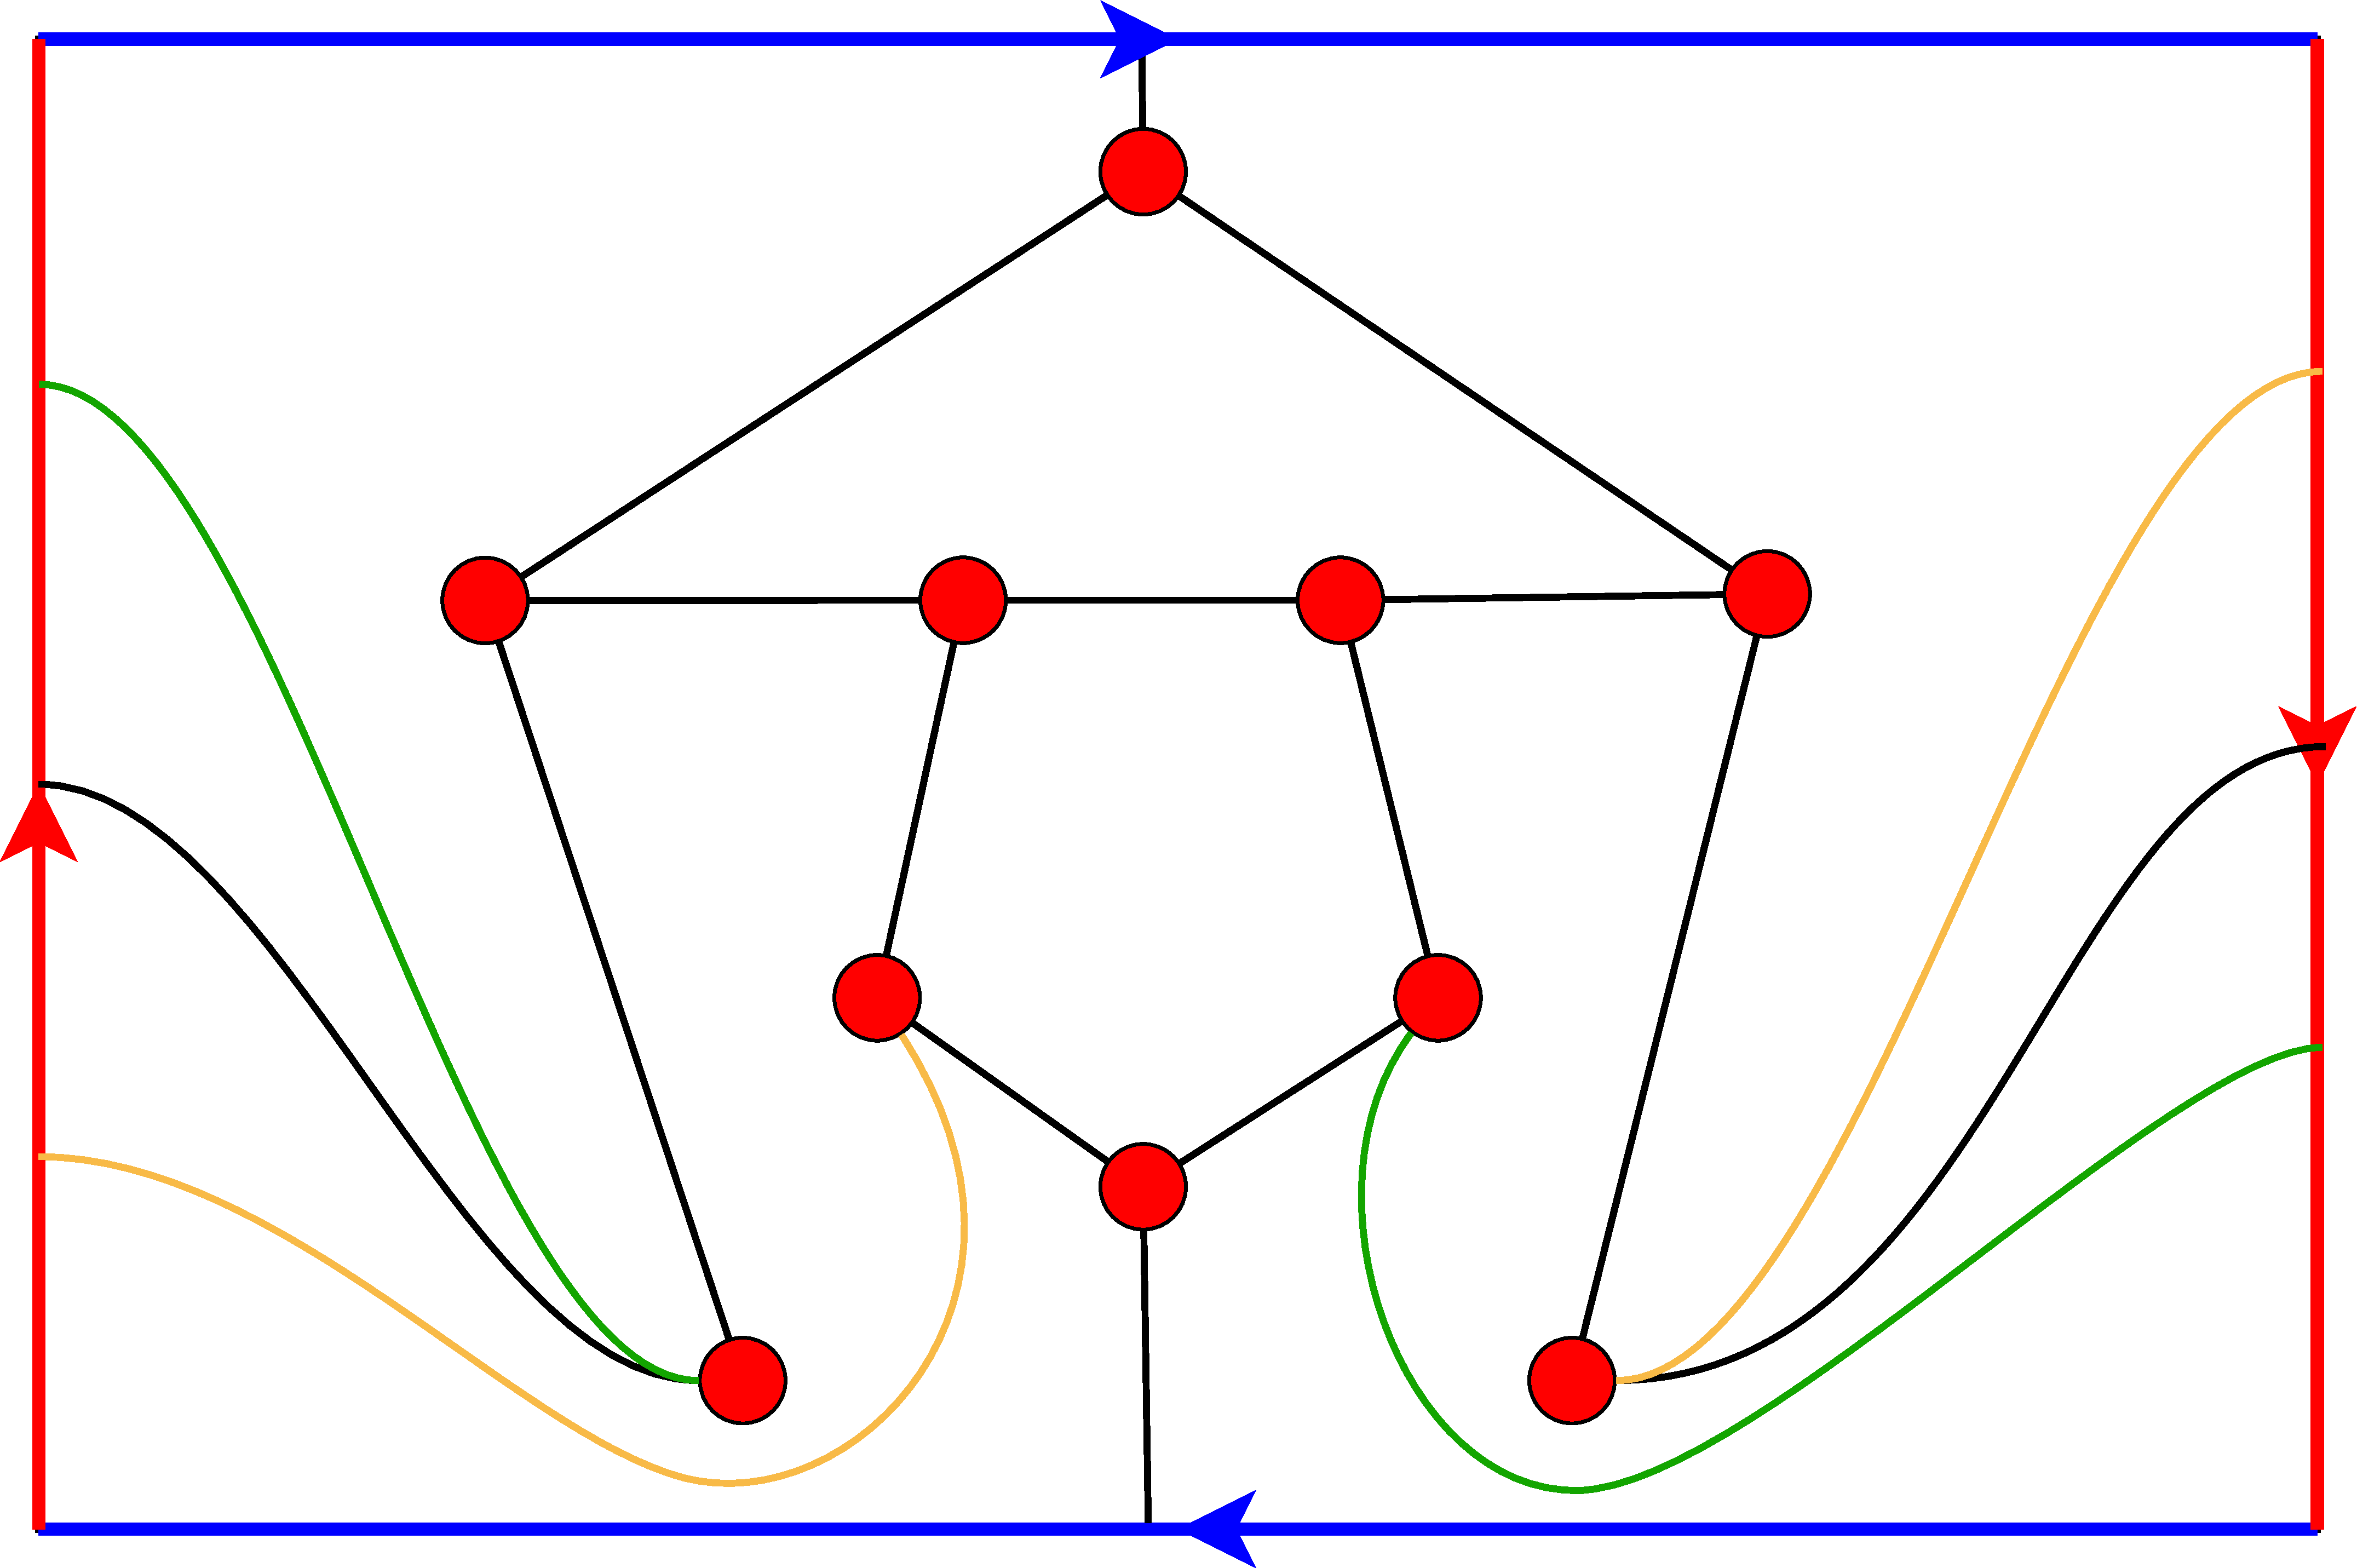
\includegraphics[keepaspectratio=true,width=0.7\textwidth]{../planar-graphs/crosscap-embedding-5.pdf}
  \caption{An embedding of the Petersen graph without edge
    intersection on the surface of the cross cap.}
  \label{fig:rp2-embedding}
\end{figure}

%%% }}}
%%%%%%%%%%%%%%%%%%%%%%%%%%%%%%%%%%%%%%%%%%%%%%%%%%%%%%%%%%%%

%%%%%%%%%%%%%%%%%%%%%%%%%%%%%%%%%%%%%%%%%%%%%%%%%%%%%%%%%%%%
%%% Bibliographieverzeichnis {{{
\newpage
\nocite{*}
\bibliographystyle{plaindin}
\bibliography{quellen}
%%% }}}
%%%%%%%%%%%%%%%%%%%%%%%%%%%%%%%%%%%%%%%%%%%%%%%%%%%%%%%%%%%%

\end{document}

%%% vim:set fdm=marker:
